
\documentclass[11pt,twoside]{article}
\usepackage{geometry}
\usepackage{enumerate}
\usepackage{latexsym,booktabs}
\usepackage{amsmath,amssymb}
\usepackage{graphicx}
\usepackage{hyperref}
\usepackage[singlespacing]{setspace}
\usepackage{calc}
\usepackage{listings}
\usepackage{xcolor}
\usepackage{float}


\definecolor{codegrey}{rgb}{0.5, 0.5, 0.5}
\definecolor{darkpurple}{RGB}{151, 10, 232}
\definecolor{backcolour}{rgb}{0.95, 0.95, 0.92}
\definecolor{forestgreen}{RGB}{5, 155, 50}
\definecolor{codeorange}{RGB}{255, 128, 0}

\lstdefinestyle{mystyle}{
    backgroundcolor=\color{backcolour},   
    commentstyle=\color{forestgreen},
    keywordstyle=\color{blue},
    numberstyle=\tiny\color{codegrey},
    identifierstyle=\color{codeorange},
    stringstyle=\color{darkpurple},
    basicstyle=\ttfamily\footnotesize,
    breakatwhitespace=false,         
    breaklines=true,                 
    captionpos=b,                    
    keepspaces=true,                 
    numbers=left,                    
    numbersep=5pt,                  
    showspaces=false,                
    showstringspaces=false,
    showtabs=false,                  
    tabsize=2
}

\lstset{style = mystyle}

\geometry{a4paper,left=2cm,right=2.0cm, top=2cm, bottom=2.0cm}

\newtheorem{Definition}{Definition}
\newtheorem{Theorem}{Theorem}
\newtheorem{Lemma}{Lemma}
\newtheorem{Corollary}{Corollary}
\newtheorem{Proposition}{Proposition}
\newtheorem{Algorithm}{Algorithm}
\numberwithin{Theorem}{section}
\numberwithin{Definition}{section}
\numberwithin{Lemma}{section}
\numberwithin{Algorithm}{section}
\numberwithin{equation}{section}

\newcommand{\dottedline}[1]{\makebox[#1]{.\dotfill}}


\begin{document}

\pagestyle{empty}

% =============================================================================
% Title page
% =============================================================================
%TC:ignore

\begin{titlepage}
\vspace*{.5em}
\center
\textbf{\Large{The School of Mathematics}} \\
\vspace*{1em}
\begin{figure}[!h]
\centering

\includegraphics[width=180pt]{CentredLogoCMYK.jpg}
\end{figure}
\vspace{2em}
\textbf{\Huge{Mimicking L'Aquila: Capturing Key Components of the Earthquake Sequence}}\\[2em]
\textbf{\LARGE{by}}\\
\vspace{2em}
\textbf{\LARGE{Robin Lin, s2435943}}\\
\vspace{6.5em}
\Large{Dissertation Presented for the Degree of\\
MSc in Statistics with Data Science}\\
\vspace{6.5em}
\Large{August 2023}\\
\vspace{3em}
\Large{Supervised by\\Dr Finn Lindgren and Dr Daniel Paulin}
\vfill
\end{titlepage}

\cleardoublepage

% =============================================================================
% Executive summary, acknowledgments, and own work declaration
% =============================================================================
\begin{center}
\Large{Executive Summary}
\end{center}

Earthquake forecasting has long been a crucial but challenging task for seismologists. Fortunately, with the help of the $\textbf{ETAS}$ model, seismologists are able to model an earthquake sequence, and obtain useful information of the sequence, such as the background rate, the average number of aftershocks, the rate of change in the aftershocks, the time offset parameter, and the decaying rate. This project aims at mimicking the L'Aquila earthquake sequence using synthetic catalogues, and investigating key characteristics of the catalogues, such as the number of events, the number of high-magnitude events, the maximum magnitude, and the time differences between $2$ consecutive events, in order to yield a better performance in resembling the real sequence in terms of the $5$ parameters mentioned above. With the help of $\textbf{\textit{R}}$ packages $\textbf{\textit{inlabru}}$ and $\textbf{\textit{ETAS.inlabru}}$ in generating and modelling the catalogues, hierarchical clustering method in sampling the representative catalogues, and eCDF and KS test plots in analysing the time differences in each catalogue, some promising results have been discovered. First, the average number of aftershocks, the time offset parameter, and the decaying rate are crucial in yielding more robust estimation results. Next, organic synthetic catalogues with $300$ to $500$ events in total, with $3$ to $5$ events of magnitudes greater than $4.5$, and with a magnitude of around $6$ in the highest event yield to better estimates of the parameters. Finally, catalogues with the L'Aquila earthquake imposed to the history have a higher chance to resemble the L'Aquila sequence in terms of time-between-events.

\clearpage

\begin{center}
\Large{Acknowledgments}
\end{center}

I would like to thank Prof. Finn Lindgren, one of my supervisors, for providing useful information such as $\textbf{\textit{R}}$ packages, instructional $\textbf{\textit{R}}$ codes, articles, and datasets, which are crucial for this project. In addition, he has been knowledgeable, and really kind and helpful in providing abundant information from $\textbf{\textit{R}}$ codes to his previous research in seismology, and from the key points of the project to some possible solutions to the problems. I really admire him, not only for his abundant academic research, but also of his meticulous and rigorous scholarship in order that I could have a clear understanding on the topic of forecasting earthquakes.

In addition, Dr. Daniel Paulin, the other supervisor, and Mr. Man Ho Suen, the PhD student helper, have been helpful in clarifying some of the key concepts that are used in this report.


\clearpage

\begin{center}
\Large{University of Edinburgh – Own Work Declaration}
\end{center}


This sheet must be filled in, signed and dated - your work will not be marked unless this is done.
\vspace{1cm}

Name: \dottedline{8cm}

Matriculation Number: \dottedline{6cm}

Title of work: \dottedline{8cm}

\vspace{1cm}

I confirm that all this work is my own except where indicated, and that I have:
\begin{itemize}
\item	Clearly referenced/listed all sources as appropriate	 				
\item	Referenced and put in inverted commas all quoted text (from books, web, etc)	
\item	Given the sources of all pictures, data etc. that are not my own				
\item	Not made any use of the report(s) or essay(s) of any other student(s) either past 	
or present	
\item	Not sought or used the help of any external professional academic agencies for the work
\item	Acknowledged in appropriate places any help that I have received from others	(e.g. fellow students, technicians, statisticians, external sources)
\item	Complied with any other plagiarism criteria specified in the Course handbook
\end{itemize}

I understand that any false claim for this work will be penalised in accordance with
the University regulations	(\url{https://teaching.maths.ed.ac.uk/main/msc-students/msc-programmes/statistics/data-science/assessment/academic-misconduct}).								

\vspace{1cm}

Signature \dottedline{8cm}

\vspace{5mm}

Date \dottedline{8cm}


\clearpage



% 


% Table of contents, tables, and pictures (if applicable)
% =============================================================================
\pagestyle{plain}
\setcounter{page}{1}
\pagenumbering{Roman}

\tableofcontents
\clearpage
\listoftables
\listoffigures
\cleardoublepage

\pagenumbering{arabic}
\setcounter{page}{1}

\nocite{*}
\bibliographystyle{abbrv}
\clearpage


%TC:endignore

\section{Introduction}
\label{sec:intro}
Earthquakes have been catastrophic, threatening people's lives. According to \cite{Earthquakes}, the global average number of deaths per year caused by earthquakes between $1998$ and $2017$ is nearly $40,000$. In order to reduce casualties and financial loss, it could be useful to design new constructions that can resist high-magnitude earthquakes, or to enhance existing constructions so that they would be resilient after such earthquakes. However, it would be way more meaningful if an ordinary person has the foresight, and they are forewarned in advance of a high-magnitude earthquake. Therefore, forecasting earthquake activities is crucial for seismologists in providing people accurate and thorough up-to-date information of when and where an earthquake would happen, how it would be like, and how it would impact people's lives, so that people would be well-prepared in coping with a possible disastrous event.

In statistics, forecasting is different from prediction. Forecasting is based on models, while prediction is based on intuition. The prediction of earthquakes has long been tough for seismologists, especially predicting an individual 
earthquake is nearly impossible for experts. According to \cite{britannicaEarthquakeDefinition}, an earthquake occurs when the seismic waves move through the crust of the earth. Such waves are usually generated when the elastic strain suddenly releases massive energy from the crust. It is extremely difficult to conduct a study on when, where, and how the energy is released, since the rocks behave stochastically inside the earth under the high temperature and pressure. This makes it hard to capture complete information of the seismic waves, which is crucial in earthquake prediction. Hence, predicting accurately the time, location, and magnitude of a possible future earthquake would hardly be practical.

Fortunately, seismologists are able to study the earthquake activities by combining geographical features with statistical modelling techniques, so as to conduct a probabilistic forecast on the possible future earthquake events on a daily basis. Essentially, the earthquake data are temporal and spatial point data, where "temporal" refers to datasets with time instances, and "spatial" refers to datasets with geographical features, such as locations and altitudes. A Poisson process model is an essential tool in modelling random events, assuming that the numbers of events occurred during any $2$ non-overlapping time intervals are independent. Data points are thus independent of each other given the conditional intensity of the process. However, an individual earthquake is likely to trigger other small earthquakes, and hence the independent assumption between events does not hold any longer. This gives rise to a process for dependent data points. Fortunately, the Hawkes process allows the possible future earthquakes to be triggered by current or previous earthquakes, so it is a suitable choice for modelling the earthquake data. Details of such a process would be discussed in later sections.

The Hawkes process model was suggested and developed in \cite{edinburghseismicityhubTemporalModeld}, \cite{naylor2023bayesian}, and  \cite{serafini2023approximation} in $2023$ by Dr. Serafini, Dr. Lindgren, and Dr. Naylor at the University of Edinburgh and the University of Newcastle, and it is also worth mentioning that some useful tools in modelling and synthetic catalogues generation are provided by them in $\textit{R}$ packages $\textit{\textbf{inlabru}}$ and $\textit{\textbf{ETAS.inlabru}}$. The aim of this project is to generate multiple synthetic catalogues, and to extract useful information of the catalogues, in order to mimic the behaviours of the real earthquake sequence, so as to help seismologists in forecasting earthquakes on a daily basis using synthetic catalogues instead of a real sequence. In order to achieve this, the true model should be constructed based on the real observed dataset. The true parameters are obtained by taking the mean of the posterior distributions of the parameters. Multiple synthetic catalogues are then generated and modelled in search of key characteristics required in an earthquake catalogue in order to resemble the true parameters. In each catalogue, such characteristics include the number of events, the number of large events, the highest magnitude, the history of events, and the inter-arrival time. For the inter-arrival time, specifically, their empirical cumulative density functions in real and synthetic earthquake catalogues are also investigated and compared in order to capture the behaviours of the arrival time of earthquake events. 

\section{Data Description}
\label{sec:data description}

Data of earthquake events are usually kept in catalogues, and the dataset used in this project is adapted from the catalogue of HOmogenised instRUmental Seismic (HORUS), containing mainly the earthquake events occurred in Italy from $1960$ to $2020$. The catalogue could be accessed in $\textit{R}$ by typing in the following command: $\textit{\textbf{ETAS.inlabru::horus}}$, and it contains the following variables.

\begin{itemize}
    \item Earthquake Event Time \textit{(\textbf{time\_string})}
    \item Longitude \textit{(\textbf{lon})}
    \item Latitude \textit{(\textbf{lat)}}
    \item Depth (in \textit{km}) \textit{(\textbf{depth})}
    \item Magnitude (in \textit{Richter Scale}) \textit{(\textbf{M})}

\end{itemize} 

According to \cite{internetgeographyLAquilaEarthquake}, a destructive earthquake hit L'Aquila, Italy on 6 April, 2009, and as a result, thousands of constructions were critically damaged, over $300$ lives were lost, and the financial loss was around US\$ $1.1$ billion. Aftershocks were also triggered, destroying transportation systems and houses. This earthquake had been the most disastrous in Italy since the 1980s. In this project, the L'Aquila sequence is to be modelled in estimating the parameters, as well as looking for factors triggering a large earthquake event. As suggested in \cite{edinburghseismicityhubTemporalModeld}, the events with magnitudes greater than $2.5$ occurred in Italy during $2009$ are considered. Hence, the cutoff magnitude $M_0$ is set to be $2.5$, the starting time $T_1$ is set to be $0$, and the end time $T_2$ is set to be $365$. The range of latitudes to be considered is between $40^\circ 30' N$ and $45^\circ N$, and that of longitudes is between $10^\circ 30' E$ and $16^\circ E$.  Within this region, $1,024$ earthquake events were recorded in $2009$. According to \cite{usgsSeverityEarthquake}, the seismic waves of an earthquake with a magnitude of over $4.5$ could be recorded by seismograph, thus the cutoff for a high-magnitude event in this project is set to be $4.5$. The total number of high-magnitude events is $14$. The following map in figure \ref{fig:italy} shows vividly the Italian earthquake locations during $2009$, as well as their magnitudes. The black dots show the events with magnitudes between $3$ and $5$, while the orange ones represent events with magnitudes between $5$ and $6$, and the red one shows the event with a magnitude greater than $6$ (which is the main shock occurred in L'Aquila). 

\begin{figure}[H]
\centering
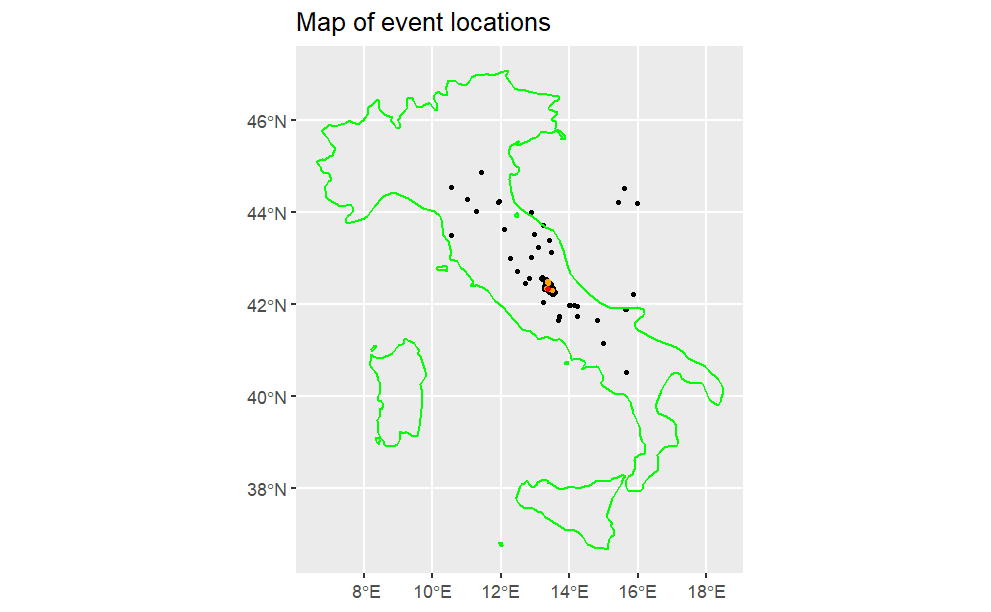
\includegraphics[scale = 1]{2/MSc_LaTeX_SwDS/MSc_LaTeX_SwDS/Italy.png}
\caption{Earthquakes in Italy near L'Aquila in 2009}
\label{fig:italy}
\end{figure}

The scatter plot shown below in figure \ref{fig:sequence} illustrates the time and magnitudes of all earthquake events occurred in 2009 near L'Aquila.

\begin{figure}[H]
\centering
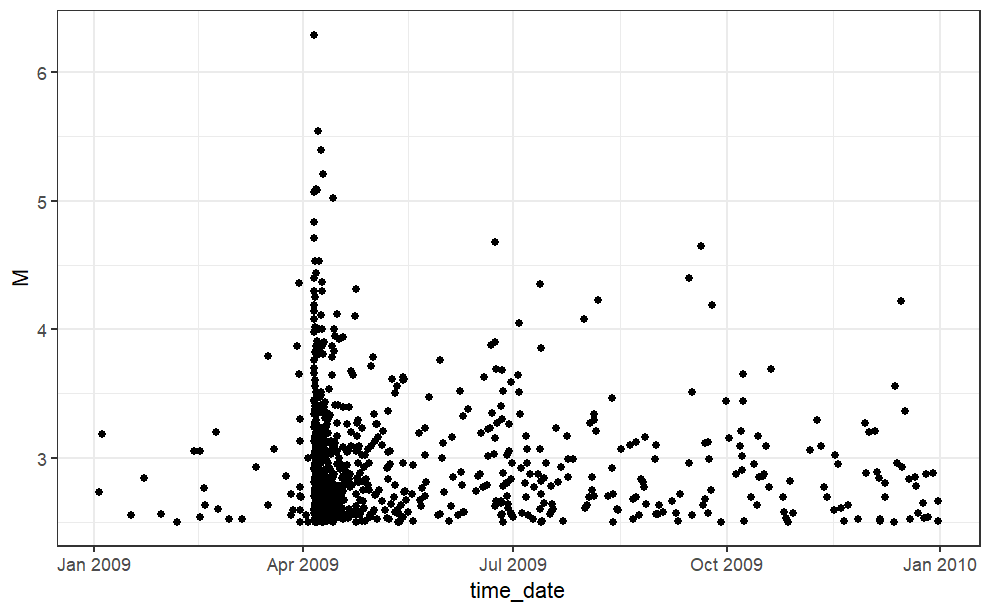
\includegraphics[scale = 1]{2/MSc_LaTeX_SwDS/MSc_LaTeX_SwDS/L'Aquila.png}
\caption{L'Aquila Sequence}
\label{fig:sequence}
\end{figure}

\section{Modelling L'Aquila Sequence}
\label{sec:Models}
\subsection{Temporal Hawkes Process}
Before the temporal and spatial data are modelled, it is crucial that the concept of a point process, and that of the Hawkes process should be well clarified. A point process is a set of points located on a space, and the temporal Hawkes process is one of the most commonly used self-exciting point processes in simulating and characterising earthquake events. Essentially, "self-exciting" describes the ability of a major event in triggering a series of small events. As suggested in \cite{edinburghseismicityhubTemporalModeld}, the conditional intensity of the temporal Hawkes process is given as follows.

\begin{equation}\label{eqn:temp_hp}
\lambda(t|\mathcal{H}_t) = \mu  + \sum\limits_{{t_h} \in {\mathcal{H}_t}} {g(t - {t_h})} 
\end{equation}

In (\ref{eqn:temp_hp}), $\mathcal{H}_t$ specifies the history of the Hawkes process before time $t$. In other words, $\mathcal{H}_t$ includes all earthquake events occurred before time $t$. $\mu$ specifies the background rate, and it is assumed to be positive. In other words, the earthquake events occur at rate $\mu$ by chance. As a triggering function of $t$, $g(t-t_h)$ characterises the intensity of a certain point process. Such a process represents the aftershocks occurred at time $t_h$, where an aftershock is the offspring of a major earthquake event. In general, a Hawkes process could be decomposed into $2$ different parts. The first part characterises the background process, and the intensity of it is $\mu$. The second part characterises a series of aftershock processes given the observed events within $\mathcal{H}_t$, and the intensity of each of them is $g(t-t_h)$. It could be seen that the Hawkes process model would be appropriate in modelling earthquake sequences, since it aims at capturing the behaviours of the offspring of the main event, and most of the time, an earthquake is likely to trigger a series of aftershocks, resembling the self-exciting process.

\subsection{Epidemic-Type Aftershock Sequence (ETAS) Model}
According to \cite{usgsPredictEarthquakes}, an earthquake event in a certain location is usually characterised by two of the key components, and they are the time point of this event, as well as the magnitude. The history of a series of earthquake events would hence be described as $\{ (t_h, m_h), h = 1, ..., N_h \}$, where $h$ represents the order of an event, $t_h$ represents the time point of this event, $m_h$ represents the magnitude of this event, and $N_h$ represents the cumulative number of events up to the time point of $t_h$. As suggested in \cite{edinburghseismicityhubTemporalModeld} and \cite{serafini2023approximation}, the Epidemic-Type Aftershock Sequence (ETAS) Model is applied in modelling the occurrences of earthquake events. The triggering function of an ETAS model is represented as follows.

\begin{equation}\label{eqn:etas_tri}
g(t-t_h)=Ke^{\alpha(m_h-M_0)}(\frac{t-t_h}{c}+1)^{-p}
\end{equation}

The conditional intensity is hence expressed as follows.


\begin{equation}\label{eqn:etas}
\lambda(t|\mathcal{H}_t) = \mu  + \sum\limits_{{t_h} \in {\mathcal{H}_t}} {Ke^{\alpha(m_h-M_0)}(\frac{t-t_h}{c}+1)^{-p}} 
\end{equation}

In (\ref{eqn:etas}), $M_0$ represents the lower bound of the magnitudes to be considered. In other words, for all $h$, $m_h \geq M_0$. In the earthquakes dataset to be modelled, $M_0$ is selected to be $2.5$. There are $5$ parameters in (\ref{eqn:etas}) to be estimated. $\mu > 0$ is the background rate, as mentioned previously. $K \geq 0$ describes the mean of aftershocks triggered by any earthquake event in the dataset. $\alpha \geq 0$ captures the changes in the number of aftershocks given the magnitude of an earthquake event triggering aftershocks. This is a scaling parameter, and such a scale should not be negative, since the higher the magnitude of an event is, the more the aftershocks it would trigger. $c>0$ is the parameter for time offset. The smaller the value is, the fewer the missing earthquake events are in the catalogues. Finally, $p>1$ describes the decaying rate of the aftershock. The parameter $p$ must have a value that is greater than $1$, since in practice, the number of aftershocks triggered are finite during a finite period of time, and if $p\le 1$, the aftershocks might not be finite, which is impractical in modelling the earthquake events. 

\subsection{Specifying Prior Distributions}
\label{subsec:prior}
In this project, the technique of Bayesian modelling is applied. Basically, the posterior distributions of $5$ of the parameters, $\mu$, $K$, $\alpha$, $c$, and $p$ are to be obtained and plotted. To achieve this, the prior distributions are to be selected. For the parameters to be estimated, it is crucial that their prior distributions are as non-informative as possible. In other words, there should not be a strong bias on the distributions of the parameters, so that the real data are able to dominate over the prior. The prior distributions were suggested in \cite{edinburghseismicityhubTemporalModeld}, and the prior distributions for the parameters $K$, $\alpha$, and $c$ are set to be the uniform distribution with a lower bound of $0$, and an upper bound of $10$, while the prior distribution for $p$ is set to be the uniform distribution with a lower bound of $1$, and an upper bound of $10$, since $p$ should be greater than $1$. The prior distribution for $\mu$ is a little bit different. Since $\mu$ is the background rate, the conditional intensity of the Hawkes process would be very high if the value of $\mu$ is large. In other words, the rate of the earthquake events would be over-estimated. According to \cite{naylor2023bayesian}, a Gamma distribution is selected for the prior of $\mu$, with a shape parameter of $0.3$, and a scale parameter of $0.6$. In this way, the density of $\mu$ would decay sharply when $\mu$ has a high value. According to \cite{naylor2023bayesian}, in the settings of the \textit{\textbf{INLA}} package, the parameters are assumed to be normally distributed, so a copula transformation is produced in order to transform a Gaussian variable into some variables of interest. Figure \ref{fig:prior_orig} shows the density curves of the simulated samples using copula transformation.
\begin{figure}[H]
\centering
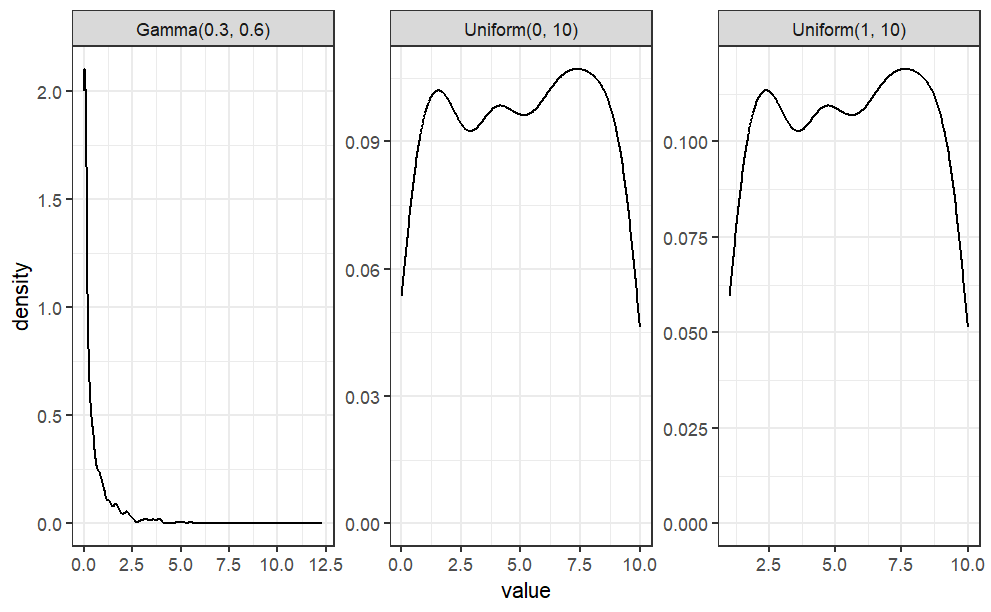
\includegraphics[scale = 1]{2/MSc_LaTeX_SwDS/MSc_LaTeX_SwDS/prior_orig.png}
\caption{Prior Distributions of the Parameters}
\label{fig:prior_orig}
\end{figure}

\subsection{Posterior Distributions of the L'Aquila Sequence}

By applying the ETAS model suggested in \cite{naylor2023bayesian} and \cite{serafini2023approximation}, the posterior distributions of the $5$ parameters are plotted, and the posterior pair plots are sketched in order to obtain the correlation between any $2$ parameters, as shown in figure \ref{fig:pair}. From the posterior plots located in the diagonal positions of figure \ref{fig:pair}, it could be observed that these distributions vary a lot from their prior distributions, showing that the real L'Aquila sequence is dominating the prior distributions in parameter estimation. In addition, by looking at the correlation coefficients, one could easily obtain that $K$ has high negative correlations with $\alpha$, $c$, and $p$, in which $c$ and $p$ have a high positive correlation. This illustrates that the more the aftershocks are triggered by an earthquake, the less changes the number of aftershocks is making, the fewer the missing events are in the catalogues, and the more slowly the decay would occur in the aftershocks. A conjecture is made, specifying that $K$ and $c$ are the $2$ parameters, of which one needs to get right in the estimation. In order to verify this, the prior distribution of one of the $5$ parameters is to be mis-specified each time, while maintaining the same prior distributions for the rest ones.
\begin{figure}[h]
\centering
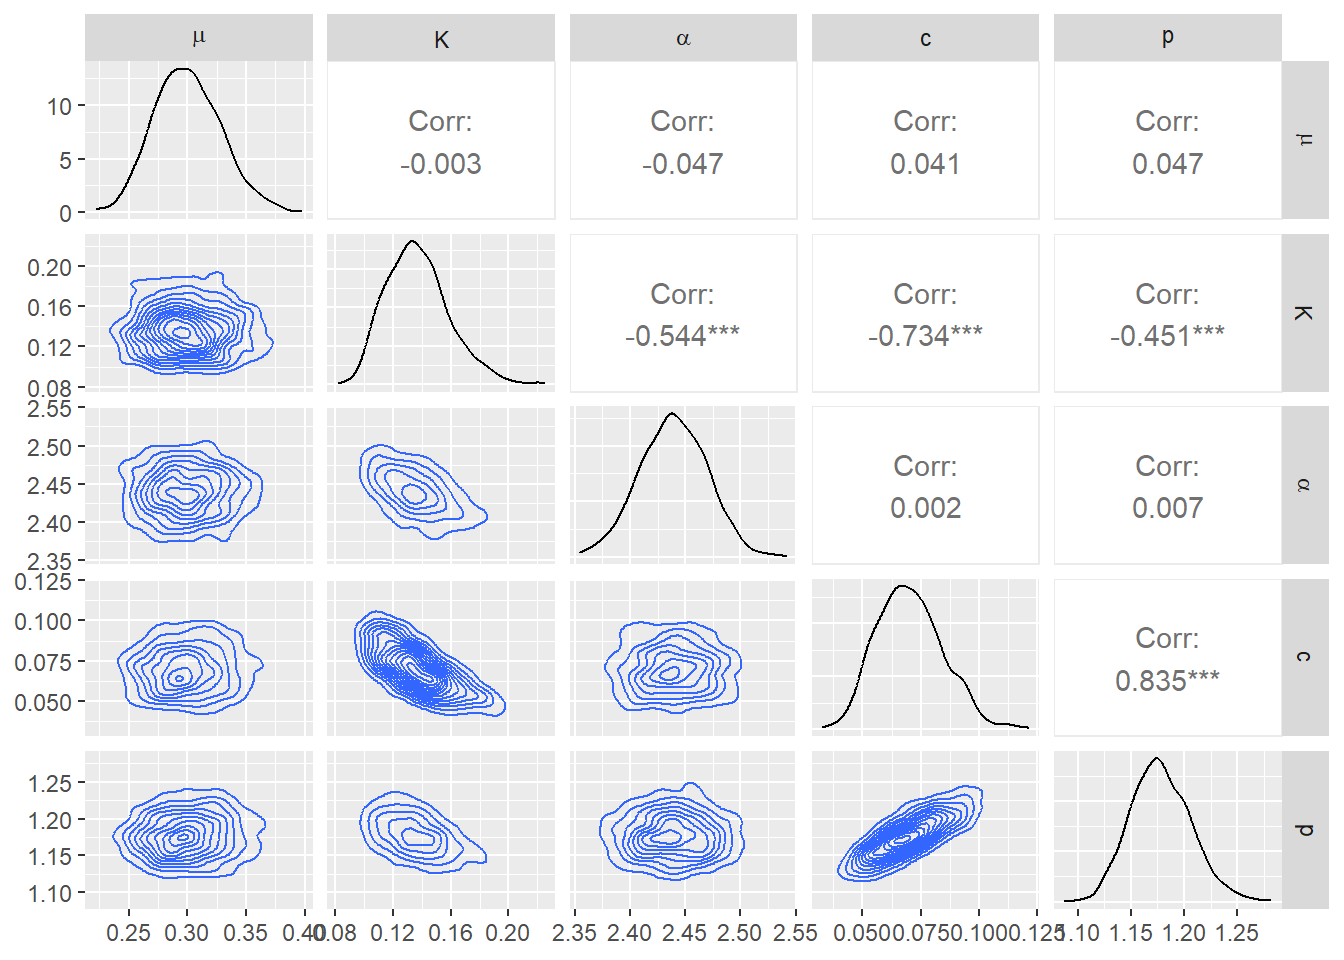
\includegraphics[scale = .8]{2/MSc_LaTeX_SwDS/MSc_LaTeX_SwDS/pairplot.png}
\caption{Pair Plots of the Posterior Parameters}
\label{fig:pair}
\end{figure}
\subsection{Mis-specifying Prior Distributions}
In this step, one of the prior distributions each time is mis-specified on purpose in their hyper-parameter values, while those values for the rest prior distributions are maintained. One would like to select distributions that are narrow in their shapes, or low in their variations, with wrong mean values that are far from those mean values of the posterior distributions obtained previously. In doing so, there would be a high bias on the prior beliefs of the mis-specified parameters, so that the posterior estimations of those parameters would be dominated by their prior distributions. In total, $5$ models are constructed, each of which with only $1$ prior distribution being mis-specified. In the first model, the prior distribution for $\mu$ is mis-specified as $Gamma(5,1)$. In the second model, the prior for $K$ is mis-specified as $Uniform(0.99,1.01)$, so does the one for $\alpha$ in the third model, and the one for $c$ in the fourth model. In the fifth model, the prior for $p$ is mis-specified as $Uniform(4.9,5.1)$. The posterior pair plots are sketched in figures \ref{fig:pair_mu} through \ref{fig:pair_p}.

\begin{figure}[h]
\centering
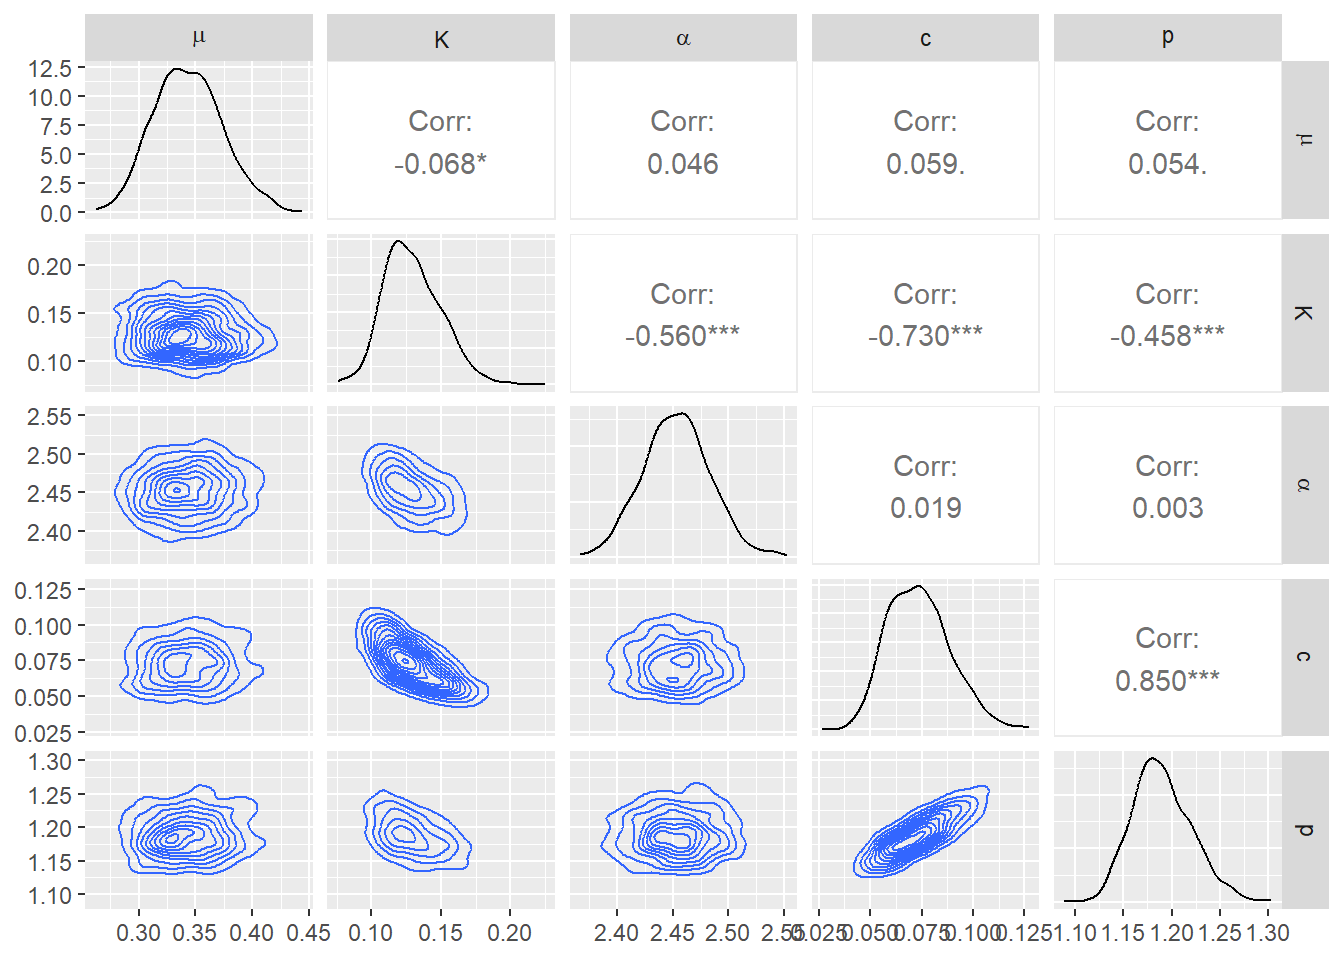
\includegraphics[scale = .8]{2/MSc_LaTeX_SwDS/MSc_LaTeX_SwDS/pairplot_mu.png}
\caption{Pair Plots of the Posterior Parameters, with $\mu$ Mis-specified}
\label{fig:pair_mu}
\end{figure}

\begin{figure}[h]
\centering
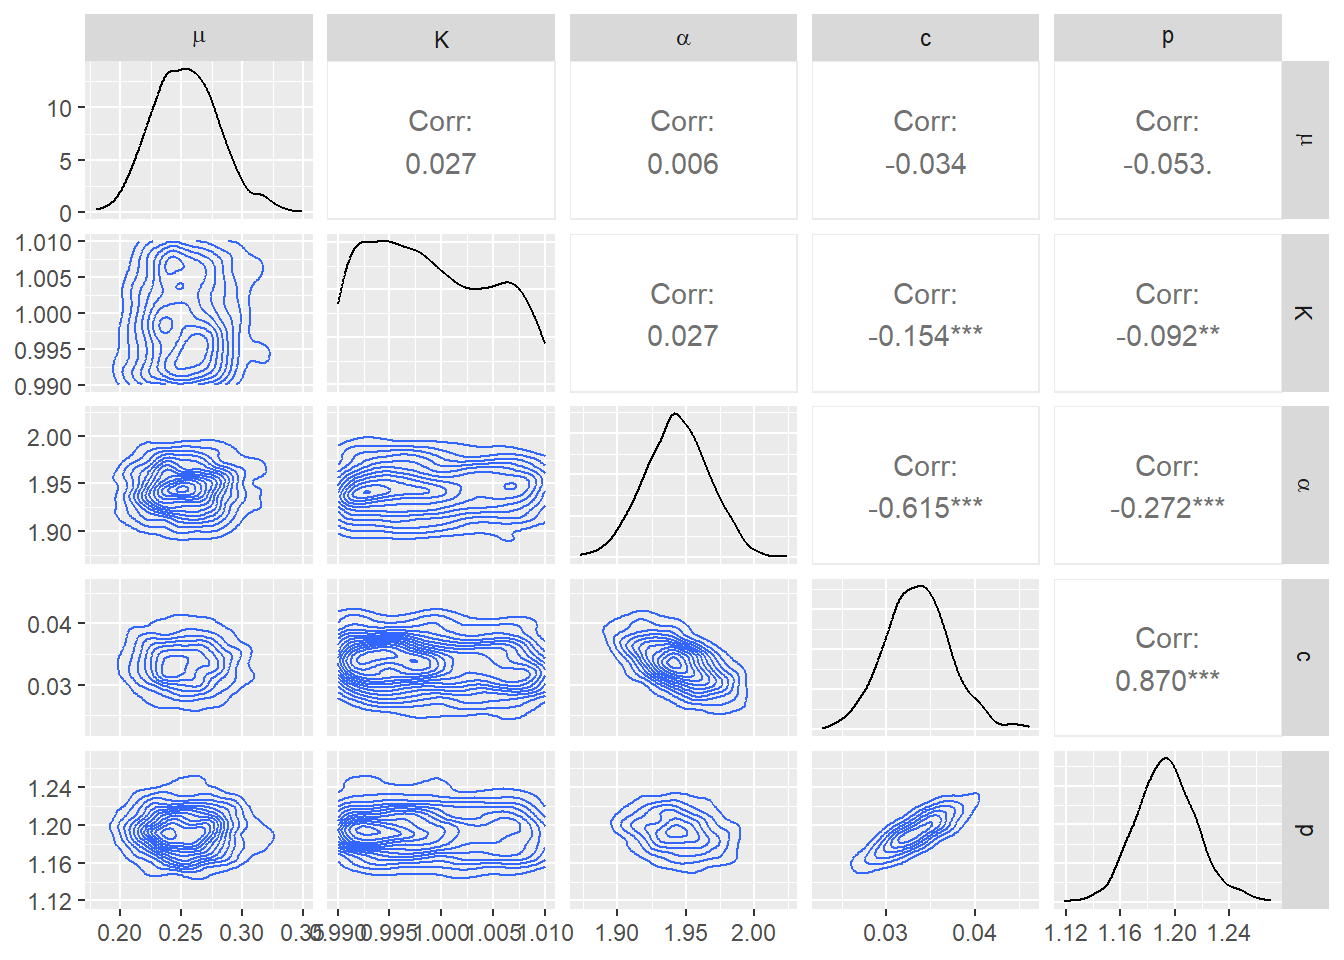
\includegraphics[scale = .8]{2/MSc_LaTeX_SwDS/MSc_LaTeX_SwDS/pairplot_K.png}
\caption{Pair Plots of the Posterior Parameters, with $K$ Mis-specified}
\label{fig:pair_K}
\end{figure}

\begin{figure}[h]
\centering
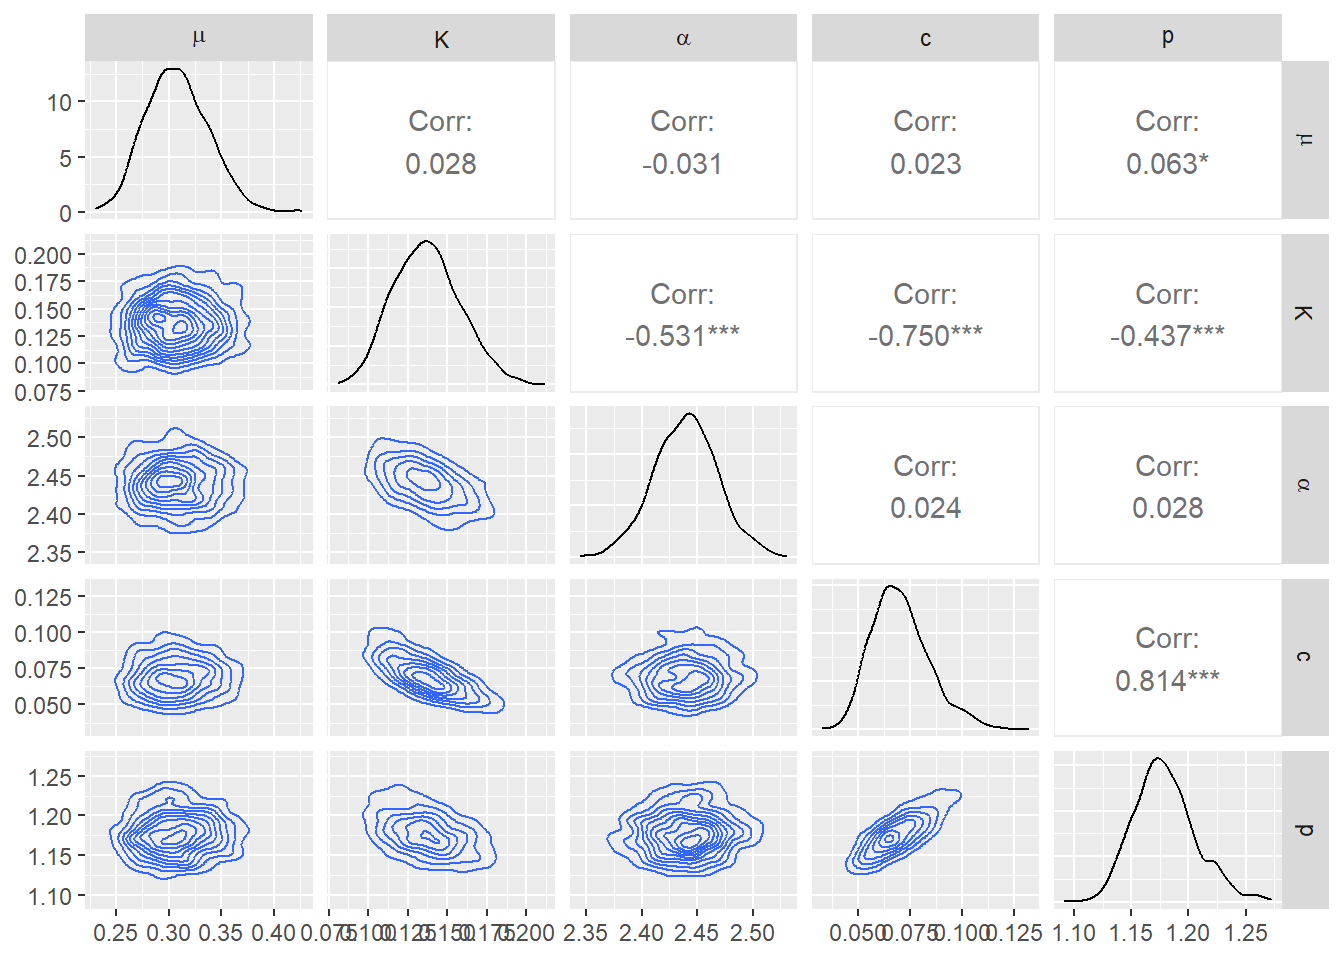
\includegraphics[scale = .8]{2/MSc_LaTeX_SwDS/MSc_LaTeX_SwDS/pairplot_alpha.png}
\caption{Pair Plots of the Posterior Parameters, with $\alpha$ Mis-specified}
\label{fig:pair_alpha}
\end{figure}

\begin{figure}[h]
\centering
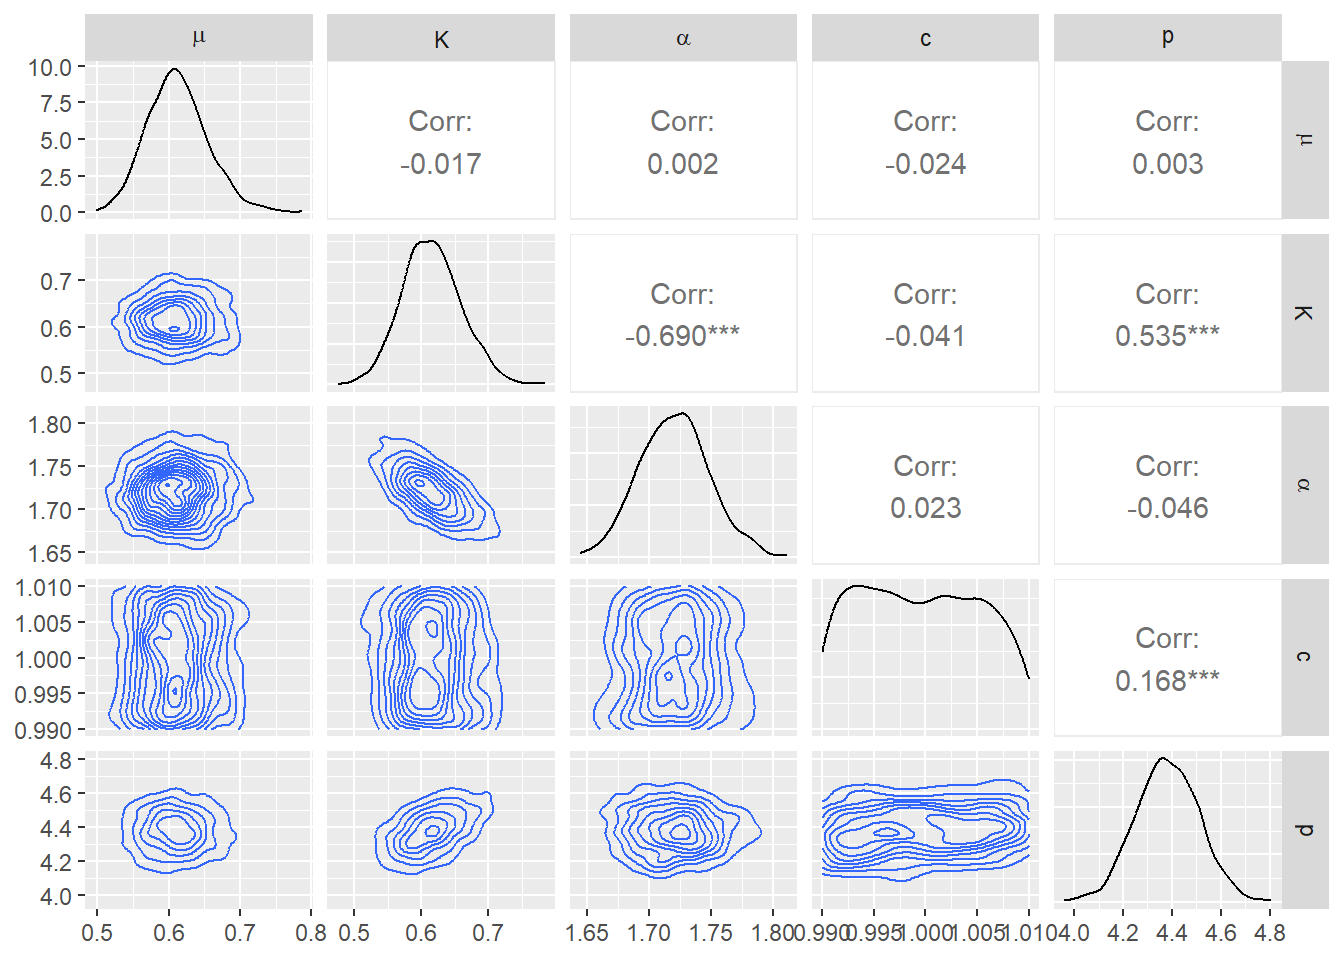
\includegraphics[scale = .8]{2/MSc_LaTeX_SwDS/MSc_LaTeX_SwDS/pairplot_c.png}
\caption{Pair Plots of the Posterior Parameters, with $c$ Mis-specified}
\label{fig:pair_c}
\end{figure}

\begin{figure}[h]
\centering
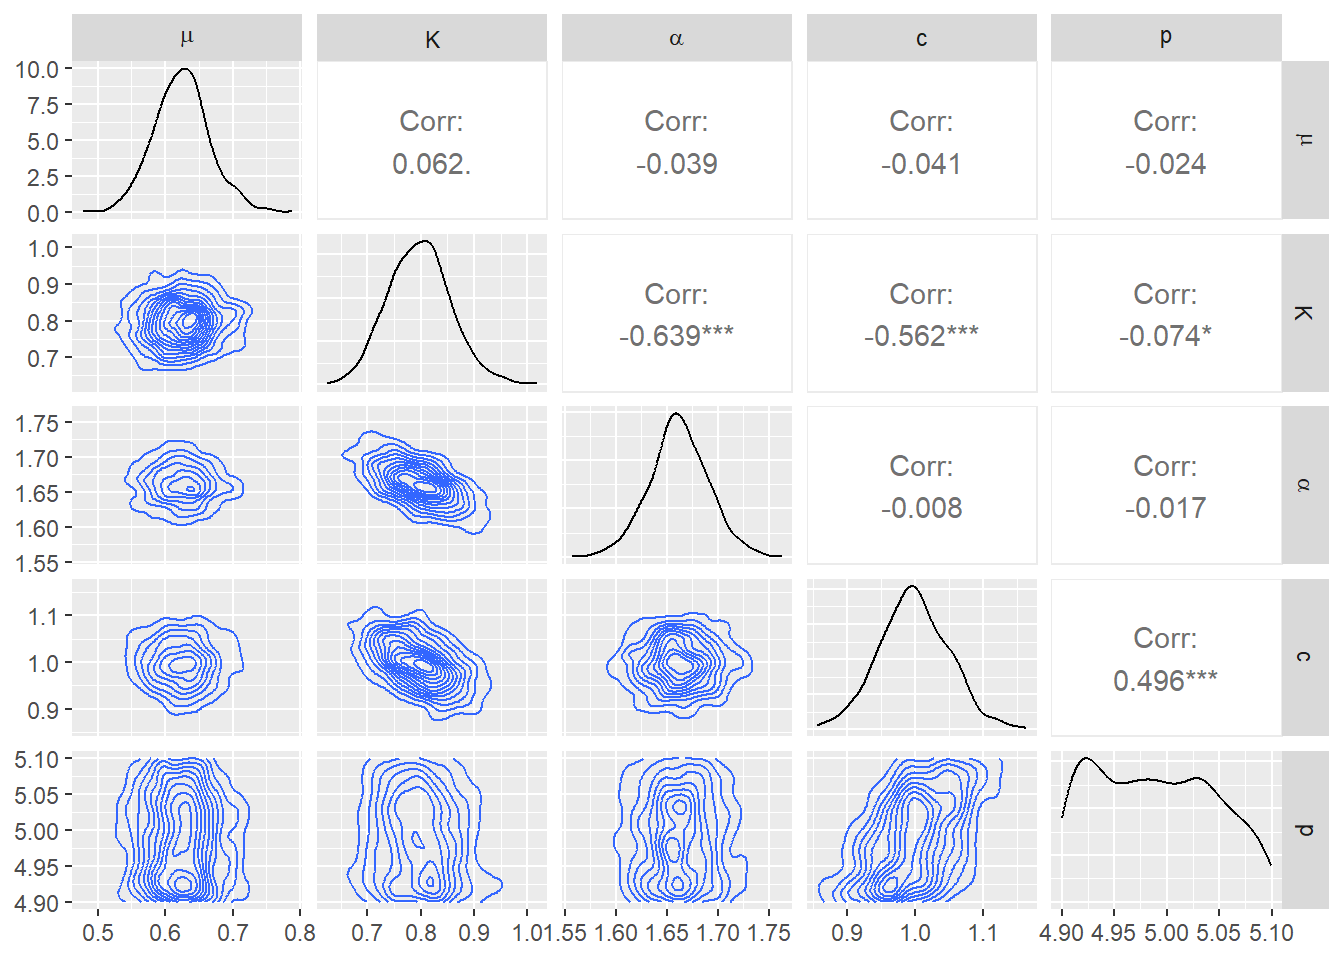
\includegraphics[scale = .8]{2/MSc_LaTeX_SwDS/MSc_LaTeX_SwDS/pairplot_p.png}
\caption{Pair Plots of the Posterior Parameters, with $p$ Mis-specified}
\label{fig:pair_p}
\end{figure}
\clearpage
From figure \ref{fig:pair_mu} to figure \ref{fig:pair_p}, one could see that mis-specifying the prior of $\mu$ or $\alpha$ would not make the posterior estimations vary a lot. However, when $K$ is mis-specified, all posterior distributions except the one for $p$ are hugely affected. Also, when $c$ or $p$ is mis-specified, all posterior distributions are hugely affected. This illustrates that one needs to get right in the prior selections of the average amount of aftershocks triggered, the time offset, as well as the decaying rate when the synthetic catalogues are generated and modelled, since the posterior estimation results would be sensitive to the prior selections of these parameters.
 
In the next section, multiple synthetic catalogues would be generated and modelled, and some of the key characteristics of the earthquake sequence would be discussed in order to mimic the behaviours of the real L'Aquila sequence.


\section{Generating and Modelling Synthetic Catalogues}
\label{sec:synth}

\subsection{Generating Catalogues}
Synthetic catalogues are crucial in earthquake forecasting, since they aim at simulating the behaviours of the real earthquake sequences. The better the performance of a synthetic catalogue resembles a sequence, the more robust the forecast would be. In order to generate the synthetic catalogues, some values are to be specified in the function $\textbf{\textit{generate\_temporal\_ETAS\_synthetic}}$ in the package $\textbf{\textit{ETAS.inlabru}}$. The first thing that one would need to determine is whether they should impose any events in generating the catalogues. When a catalogue is being generated without imposing any events, it is regarded in this paper as an \textit{organic} catalogue. When the Hawkes process model is applied to a synthetic catalogue, it is better for the catalogue to be organic than to be unnatural. As mentioned in the previous section, the Hawkes process is a self-exciting one, meaning that the earthquakes would be generated over and over again if some events are imposed, increasing the total number of events in a catalogue unrealistically. For example, if one imposes an event with the highest magnitude to the history, the number of events generated in some catalogues would be more than $4,000$, which is not realistic for the Europe to have this amount of earthquakes within a year. Also, it would be computationally intensive to construct models having this amount of events. Therefore, in this paper, organic catalogues are considered in modelling them.

In addition, some of the parameters are needed to be determined, including the $5$ parameters mentioned above, as well as the magnitude distribution parameter $\beta$. According to \cite{edinburghseismicityhubTemporalModeld}, the empirically estimated value of parameter $\beta$ obtained by using the maximum likelihood estimation is determined by taking the reciprocal of the difference between the mean of the magnitudes and the cutoff magnitude, $i.e.$, 
\begin{equation}\label{eqn:beta}
\hat \beta  = \frac{1}{{mean(magnitudes) - {M_0}}}
\end{equation}
 
For the $5$ parameters specified in previous sections, the values selected for generating catalogues should be the mean values of their own posterior samples. In summary, the parameters have the values as follows.
\begin{table}[h]
\centering
\begin{tabular}{|c|c|c|c|c|c|}

\hline
$\mu$   & K    & $\alpha$  & c    & p    & $\beta$ \\ \hline
0.30 & 0.14 & 2.44 & 0.07 & 1.18 & 2.35 \\ \hline

\end{tabular}
\caption{Parameters for Catalogues Generation}
\label{tab:parcat}

\end{table}

In this project, $1000$ synthetic catalogues are generated in order to mimic the real L'Aquila sequence in terms of key characteristics including the number of events, the number of large events, and the maximum magnitudes of the catalogues. However, fitting $1000$ models is computationally intensive, and thus some representative catalogues should be sampled, which would be discussed next.

\subsection{Hierarchical Clustering}
In order to obtain the representative samples, hierarchical clustering method is applied. In statistics, a cluster is a subset of samples, of which the elements are less distinct than the samples that are not in this subset. The main goal of clustering is to obtain the most distinct groups, so that when the same number of samples come from different clusters, these samples would be diverse, representing the major behaviours of the catalogues. There are a bunch of clustering algorithms, including K-means clustering, as well as hierarchical clustering. In this project, hierarchical clustering is adopted, since the number of clusters is not required to be predefined. Basically, hierarchical clustering groups the data points recursively based on the most appropriate linkage method in measuring how distinct the groups are. There are $4$ linkage methods in measuring the distinctions between groups, and they are single linkage, complete linkage, average linkage, as well as Ward linkage. The agglomerative coefficient, representing the strength of the structure of clusters, is computed for each of the $4$ methods, and the one with the highest coefficient is selected as the most appropriate linkage method. Next, a good measure of distances is to be determined. In this paper, the Euclidean distance is applied. Finally, the clustering gap statistic, measuring how good the clusters are, is computed in search of the optimal number of clusters with the highest value of such statistic. The dendrogram of the clustered catalogues is shown as follows in figure \ref{fig:dendro}.

\begin{figure}[h]
\centering
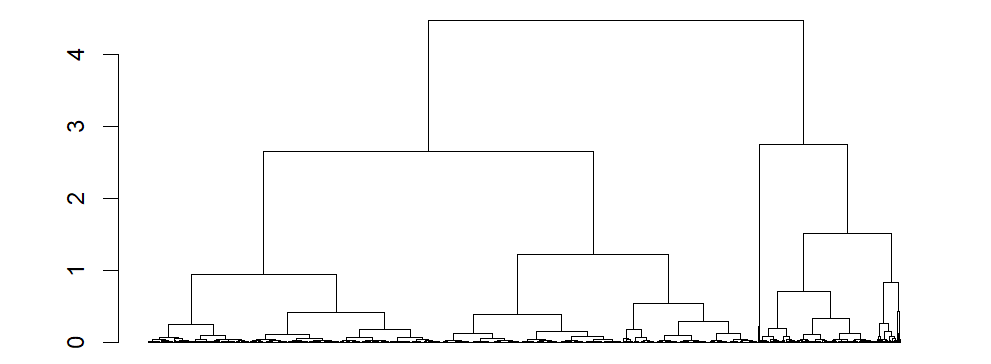
\includegraphics[scale = 1]{2/MSc_LaTeX_SwDS/MSc_LaTeX_SwDS/dendro.png}
\caption{Dendrogram of the Clustered Catalogues}
\label{fig:dendro}
\end{figure}

\subsection{Sampling and Modelling}
After generating the synthetic catalogues, a $3$-dimensional characteristic vector is obtained for each catalogue, containing information about the number of events, the number of large events, as well as the maximum magnitude. In total, $1000$ characteristic vectors are generated. These vectors are then grouped into $25$ clusters using hierarchical clustering. Figure \ref{fig:3d}  illustrates vividly the scatter plot of the characteristics, with different colours of points representing different catalogues. For most of the organic catalogues, the number of events, and that of large events is small. Regardless of some outliers, most of the catalogues have a few hundred events, with less than $10$ large events, and the maximum magnitudes lie between $4$ and $6$. 

\begin{figure}[h]
\centering
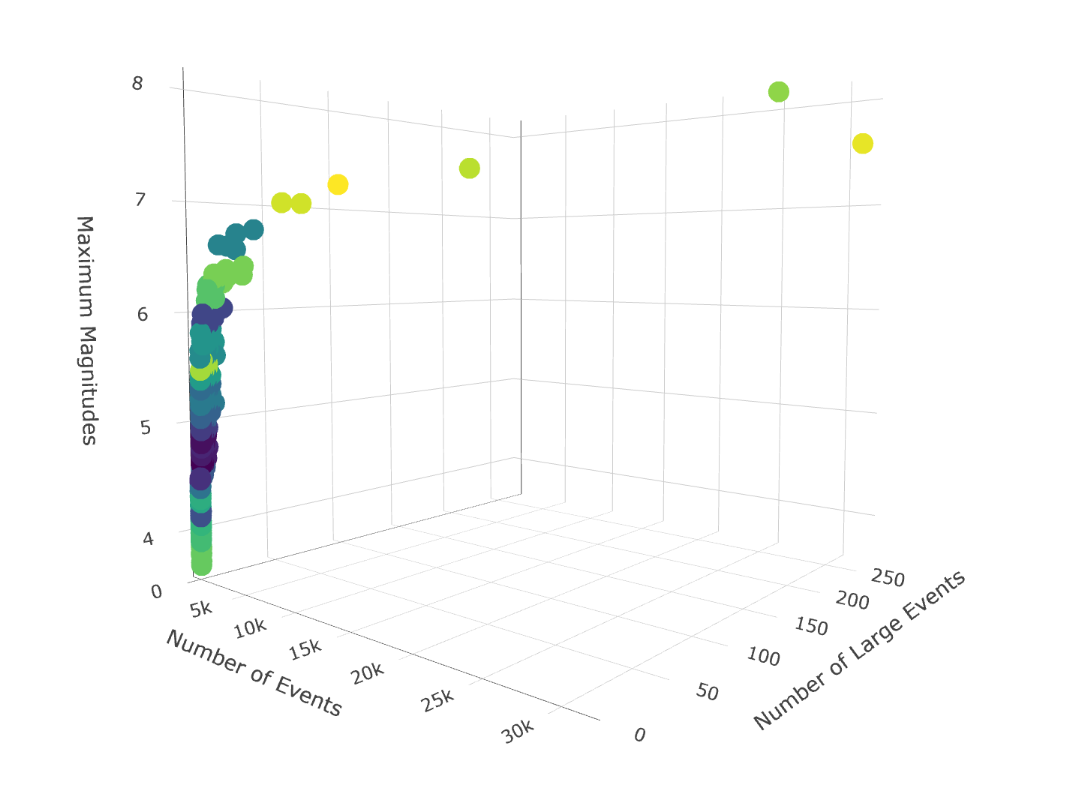
\includegraphics[scale = .7]{2/MSc_LaTeX_SwDS/MSc_LaTeX_SwDS/cluster3d.png}
\caption{3D Scatter Plot of the Clustered Catalogues}
\label{fig:3d}
\end{figure}

After the clusters are obtained, $1$ catalogue is sampled from each of the $25$ clusters, and models are then constructed, using the same prior distributions in section \ref{subsec:prior}. The plots of the sampled catalogues are in figures \ref{fig:syn1} through \ref{fig:syn3}. Totally there would be $25$ models, with random catalogues selected. The posterior parameter plots are shown in the plots in figures \ref{fig:synfit1} through \ref{fig:synfit3}.

Previously, the sensitivity of the parameters was discussed, specifying that the number of aftershocks, the time offset parameter, and the decaying rate are to be estimated correctly in order to provide a better estimation of the other parameters. From the figures of the posterior plots, it could be observed that the posterior distributions of the sequence with $300$ to $500$ total events, with $3$ to $5$ large events, and with the largest event of magnitude around $6$ would lead to better estimates of these $3$ parameters, yielding more robust estimation results of the other $2$ parameters.


\begin{figure}[H]
\centering
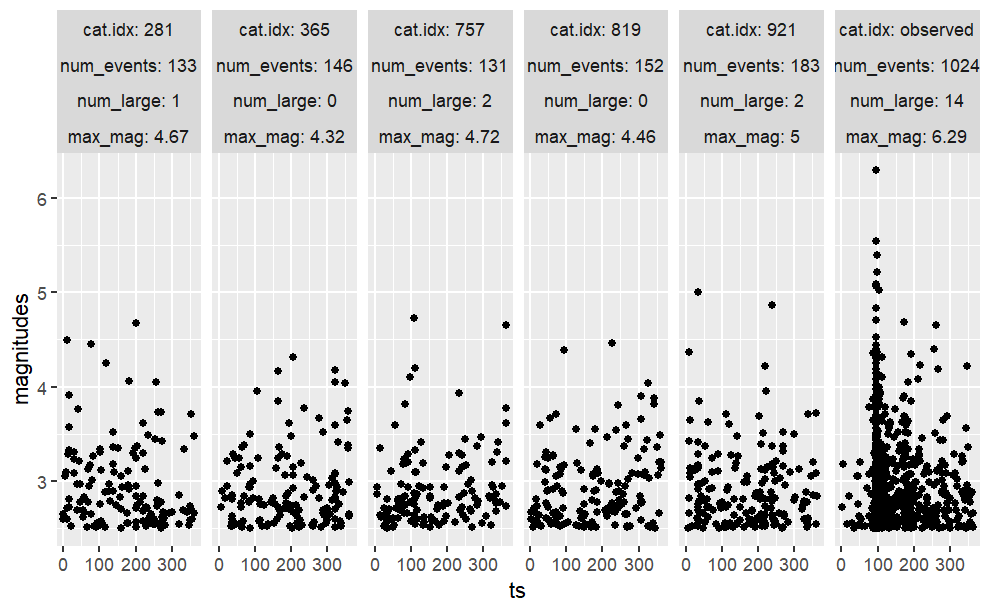
\includegraphics[scale = 1]{2/MSc_LaTeX_SwDS/MSc_LaTeX_SwDS/syn1.png}
\caption{Synthetic Catalogues (1)}
\label{fig:syn1}
\end{figure}

\begin{figure}[H]
\centering
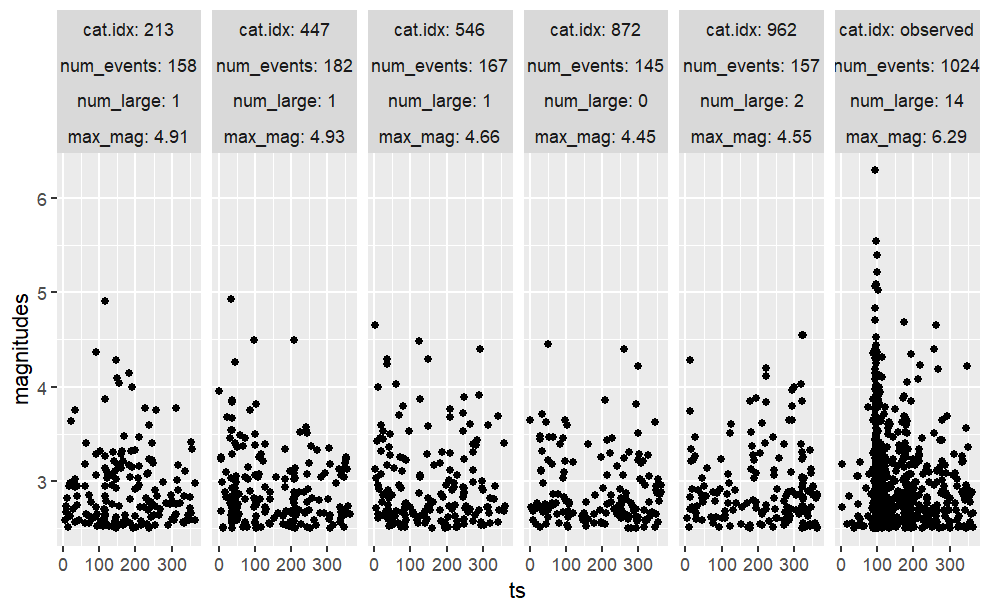
\includegraphics[scale = 1]{2/MSc_LaTeX_SwDS/MSc_LaTeX_SwDS/syn2.png}
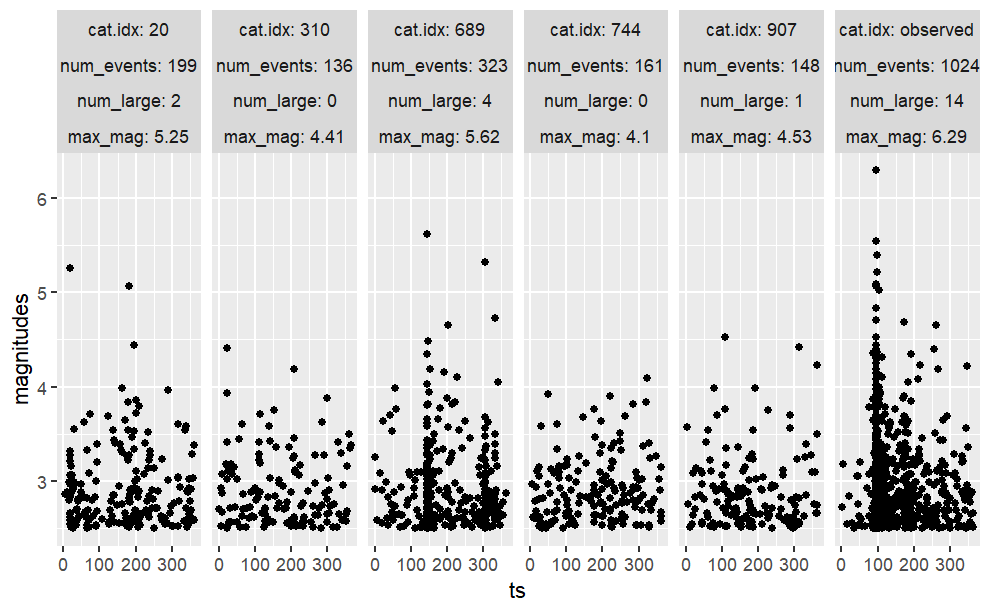
\includegraphics[scale = 1]{2/MSc_LaTeX_SwDS/MSc_LaTeX_SwDS/syn3.png}
\caption{Synthetic Catalogues (2)}
\label{fig:syn2}
\end{figure}

\begin{figure}[H]
\centering
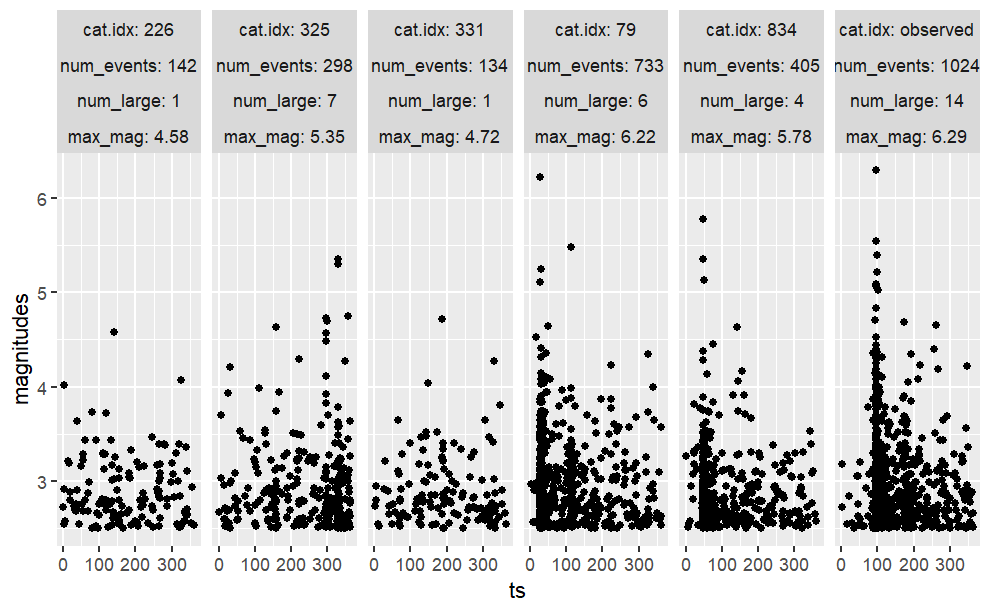
\includegraphics[scale = 1]{2/MSc_LaTeX_SwDS/MSc_LaTeX_SwDS/syn4.png}
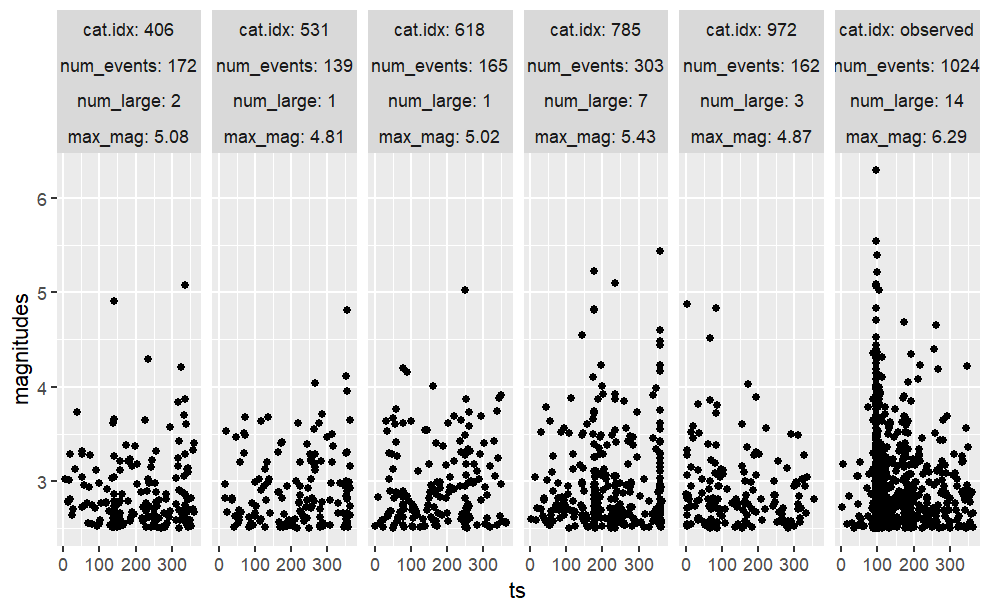
\includegraphics[scale = 1]{2/MSc_LaTeX_SwDS/MSc_LaTeX_SwDS/syn5.png}
\caption{Synthetic Catalogues (3)}
\label{fig:syn3}
\end{figure}



\begin{figure}[H]
\centering
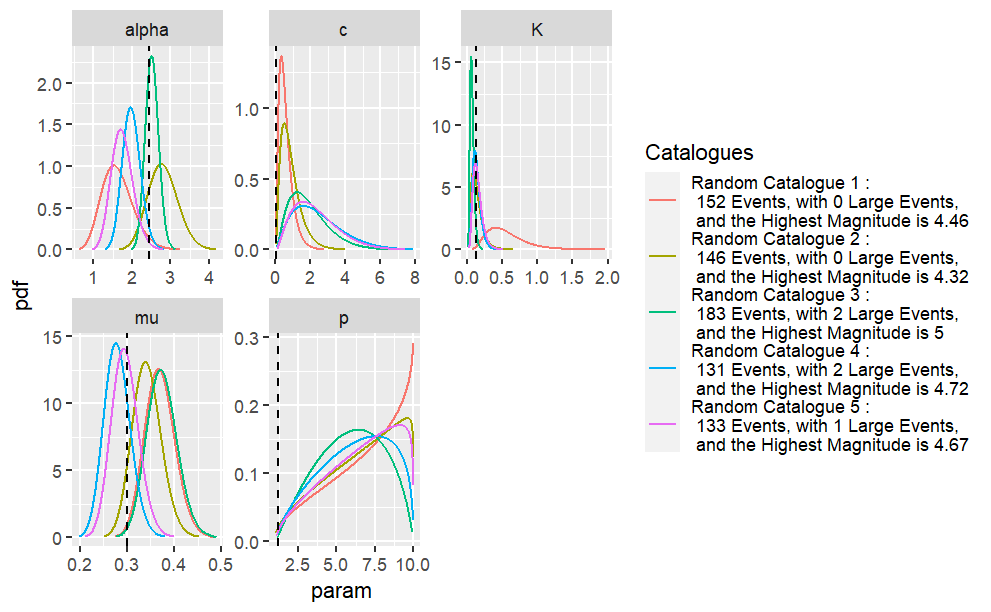
\includegraphics[scale = 1]{2/MSc_LaTeX_SwDS/MSc_LaTeX_SwDS/synfit1.png}
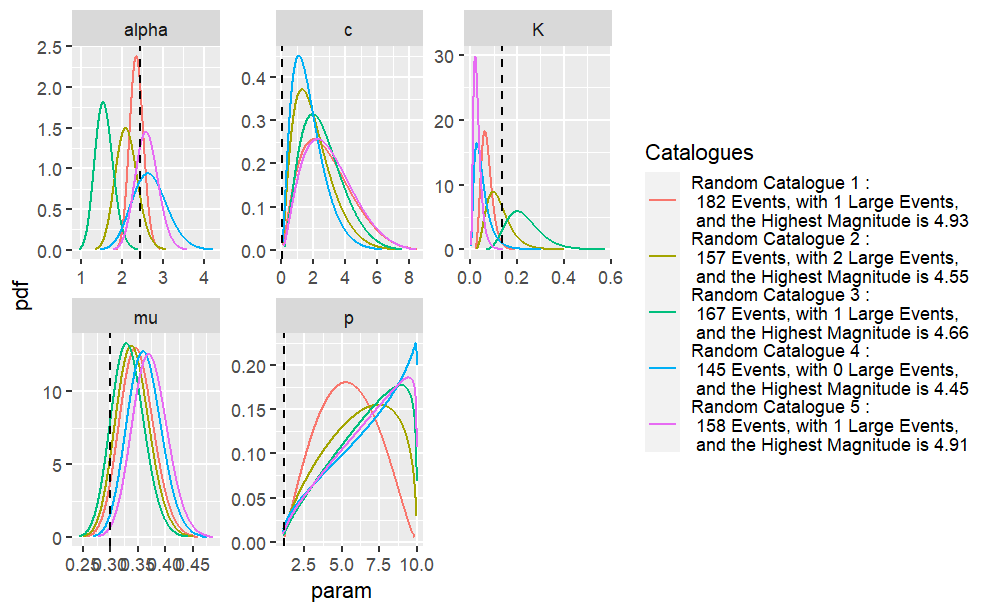
\includegraphics[scale = 1]{2/MSc_LaTeX_SwDS/MSc_LaTeX_SwDS/synfit2.png}
\caption{Posterior Plots of the Synthetic Catalogues (1)}
\label{fig:synfit1}
\end{figure}

\begin{figure}[H]
\centering
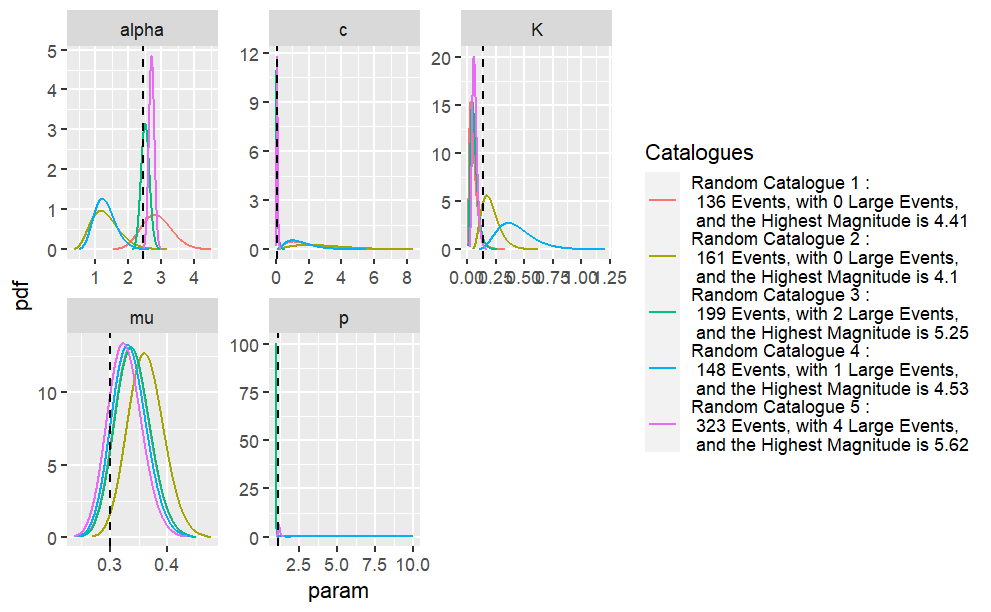
\includegraphics[scale = 1]{2/MSc_LaTeX_SwDS/MSc_LaTeX_SwDS/synfit3.png}
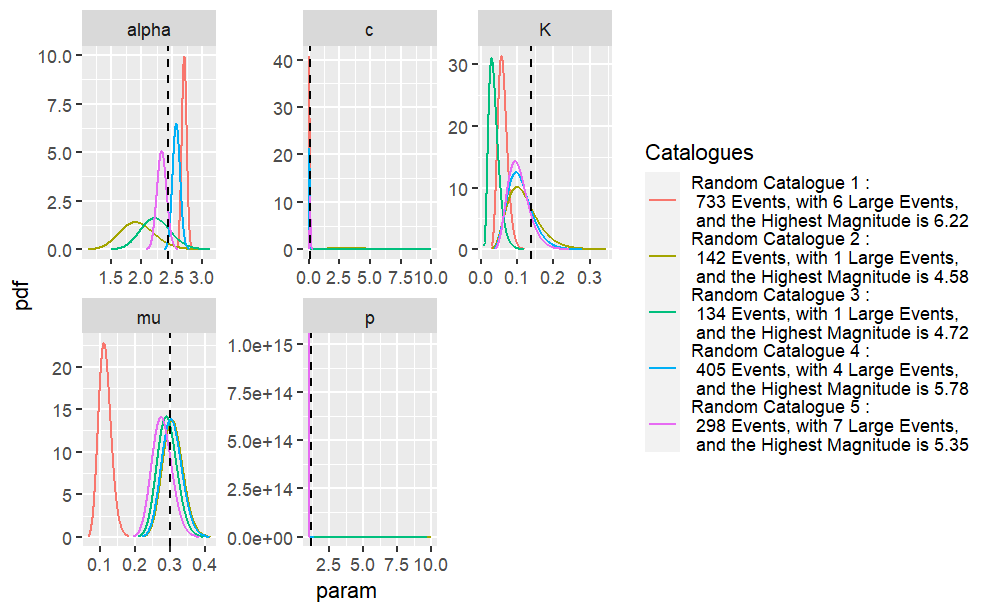
\includegraphics[scale = 1]{2/MSc_LaTeX_SwDS/MSc_LaTeX_SwDS/synfit4.png}
\caption{Posterior Plots of the Synthetic Catalogues (2)}
\label{fig:synfit2}
\end{figure}

\begin{figure}[H]
\centering
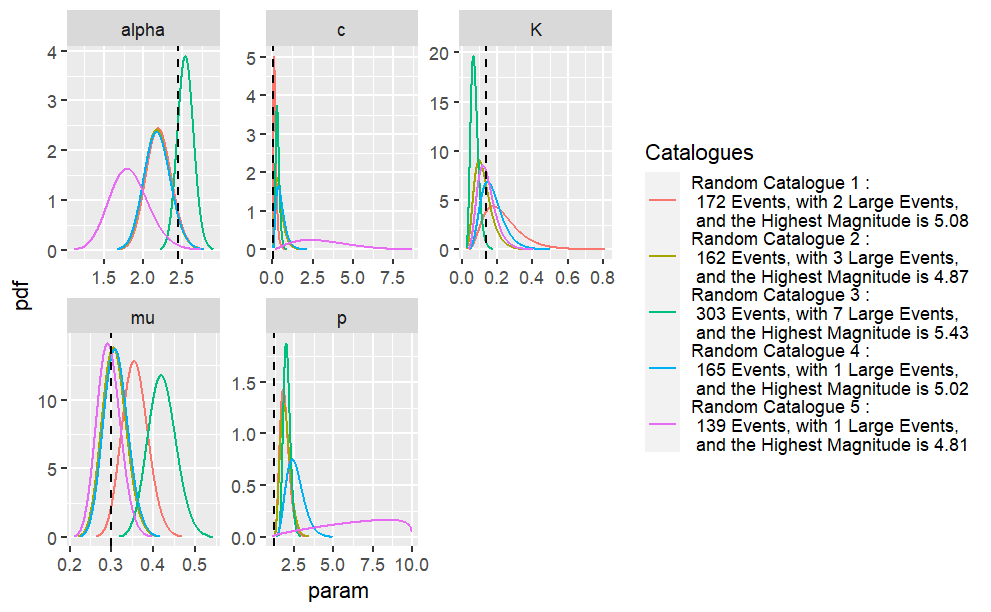
\includegraphics[scale = 1]{2/MSc_LaTeX_SwDS/MSc_LaTeX_SwDS/synfit5.png}
\caption{Posterior Plots of the Synthetic Catalogues (3)}
\label{fig:synfit3}
\end{figure}



\section{Analysis on the Time-between-Events}
\subsection{Comparing the Empirical Cumulative Density Functions (ECDF)}
Finally, the time-between-events in the synthetic catalogues and the real sequence are being investigated. For the $25$ organic catalogues selected above, the empirical cumulative density functions (eCDF) of the synthetic catalogues and the real sequence are being plotted. To clarify, an eCDF of $n$ $i.i.d.$ samples $\{X_1,...,X_n\}$ is defined as follows.

\begin{equation}\label{eqn:ecdf}
\hat F_n (t) = \frac{1}{n}\sum\limits_{i = 1}^n {{\rm I}({X_i} \le t)}
\end{equation}
\noindent
where $I(\cdot)$ represents the indicator function. In other words, the cumulative density at time $t$ is estimated as the total proportion of events occurred before time $t$. By comparing the eCDF of each of the synthetic catalogues as well as the real sequence, one could tell whether the synthetic catalogues mimic the real L'Aquila sequence well in terms of the time-between-events. Figures \ref{fig:ecdf1}  through \ref{fig:ecdf3}  illustrates the comparison of eCDF between the synthetic catalogues and the real sequence. It could be observed that as the number of events goes higher, the time-between-events of the synthetic catalogues mimic those of the real L'Aquila sequence. It is of one's interest whether a higher number of total events would lead to a better similarity in the distribution. The main event of the L'Aquila sequence, which is the L'Aquila earthquake, is then being imposed to the history, so that there would be more earthquakes being triggered. As shown in figure \ref{fig:ecdf_imp}, the numbers of events in the catalogues are generally higher, and the catalogues generated perform much better in simulating the real sequence. In order to obtain how much better the catalogues perform, the Kolmogorov-Smirnov (KS) test plots are sketched. 

\begin{figure}[H]
\centering
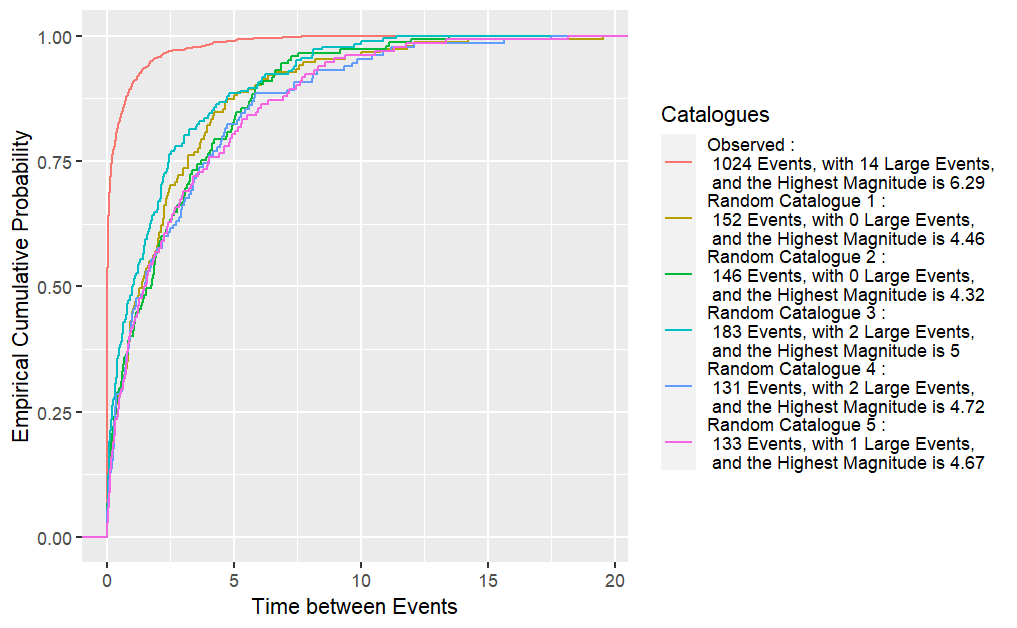
\includegraphics[scale = 1]{2/MSc_LaTeX_SwDS/MSc_LaTeX_SwDS/ecdf1.png}
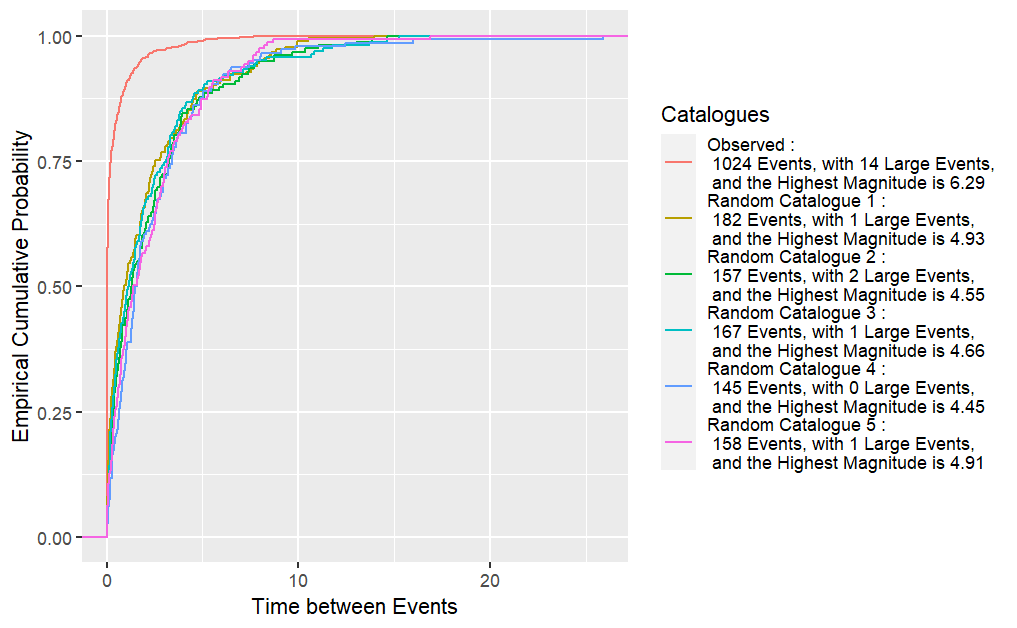
\includegraphics[scale = 1]{2/MSc_LaTeX_SwDS/MSc_LaTeX_SwDS/ecdf2.png}

\caption{ECDF of the Time-between-Events, Organic Catalogues(1)}
\label{fig:ecdf1}
\end{figure}

\begin{figure}[H]
\centering

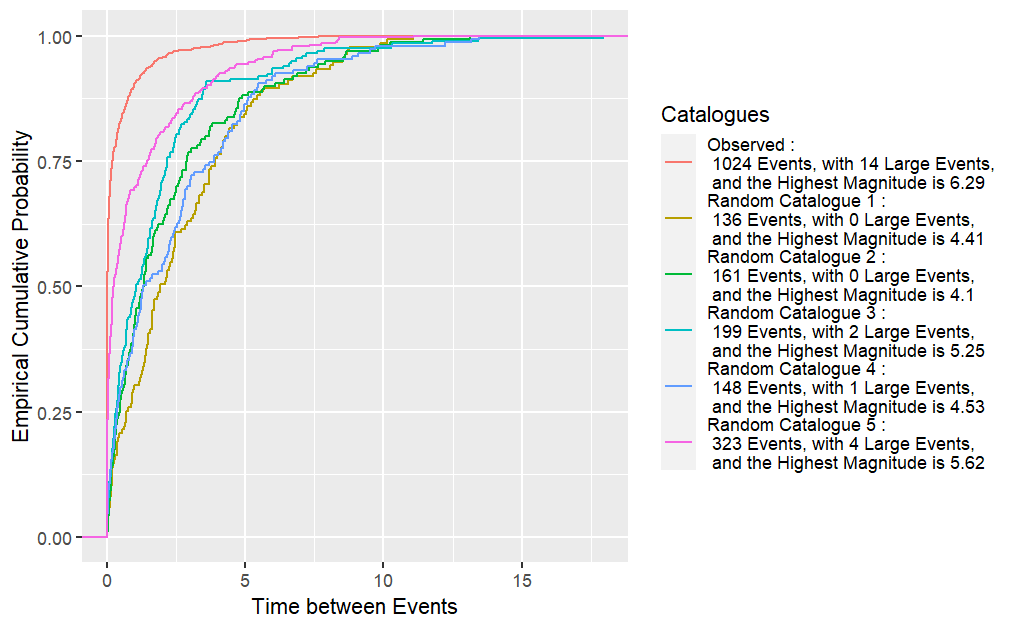
\includegraphics[scale = 1]{2/MSc_LaTeX_SwDS/MSc_LaTeX_SwDS/ecdf3.png}
\caption{ECDF of the Time-between-Events, Organic Catalogues(2)}
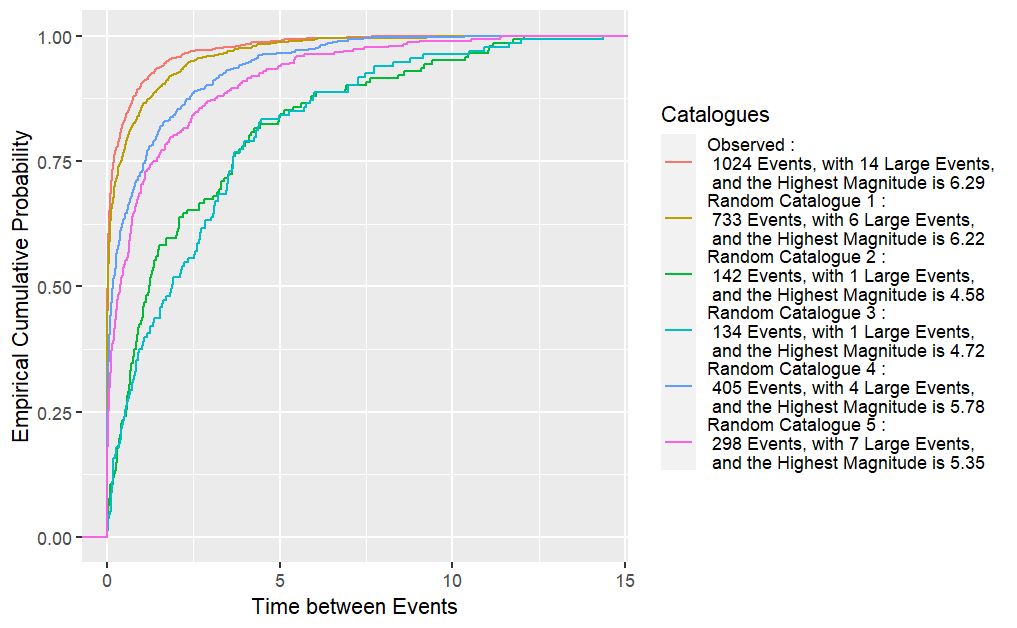
\includegraphics[scale = 1]{2/MSc_LaTeX_SwDS/MSc_LaTeX_SwDS/ecdf4.png}

\label{fig:ecdf2}
\end{figure}

\begin{figure}[H]
\centering

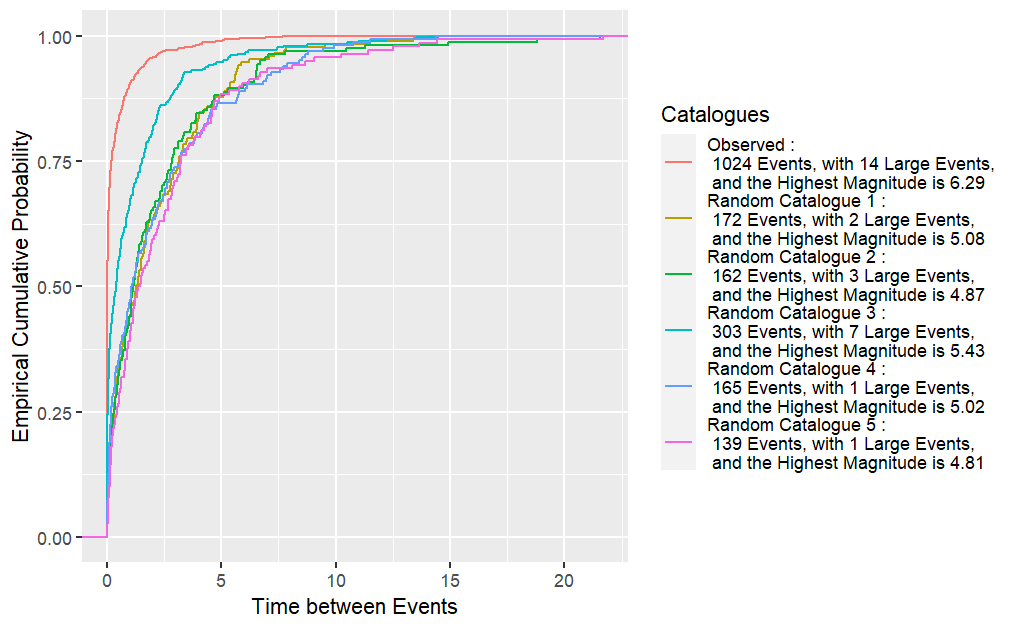
\includegraphics[scale = 1]{2/MSc_LaTeX_SwDS/MSc_LaTeX_SwDS/ecdf5.png}
\caption{ECDF of the Time-between-Events, Organic Catalogues(3)}
\label{fig:ecdf3}
\end{figure}

\begin{figure}[H]
\centering
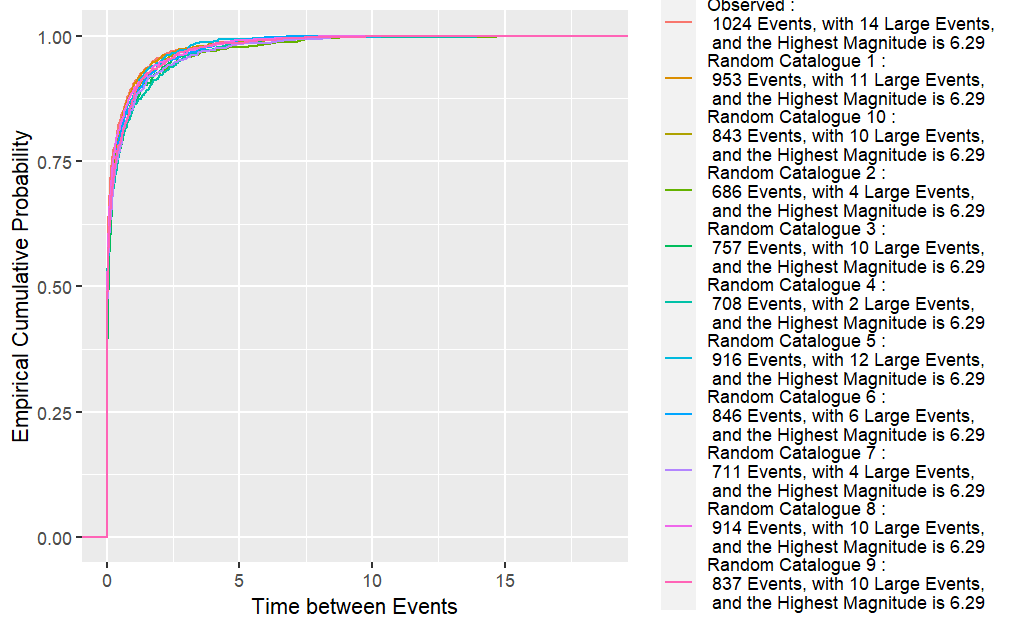
\includegraphics[scale = 1]{2/MSc_LaTeX_SwDS/MSc_LaTeX_SwDS/ecdf_imp.png}
\caption{ECDF of the Time-between-Events, Catalogues with Imposed History}
\label{fig:ecdf_imp}
\end{figure}

\subsection{Kolmogorov-Smirnov (KS) Test Plots}
In statistics, a Komolgorov-Smirnov (KS) test aims at testing whether the data follows a certain distribution. The null hypothesis is that the data follow some distribution, and a larger p-value indicates a stronger similarity in their behaviours. In the $\textbf{\textit{R}}$ package $\textbf{\textit{INLA}}$, the $\textbf{\textit{inla.ks.plot}}$ function, written by Dr. Lindgren, is applied in this project in obtaining the KS test plots. If a data curve has most of the parts falling into the ellipse, a good model fit is indicated. In the following plots, the winding curve represents the behaviour of one of the synthetic catalogues, compared with the baseline of the real sequence, which is represented by an ellipse. Figure \ref{fig:ks_org} represents the behaviour of time-between-events of an organic catalogue with the best performance, and figure \ref{fig:ks_imp} represents the behaviour of time-between-events of a catalogue with imposed history, also with the best performance. As shown in the figures, the KS plot of time-between-events of the catalogue with history imposed performs way better than the organic one, indicating that the catalogue with imposed event is able to capture the arrival time, and mimic the real sequence in a much better way. However, one should be very careful with the choice of history being imposed, since it is not necessarily the better the performance it would produce as the number of events increases. In general, catalogues having similar number of events, similar number of large events, as well as the similar highest magnitude with the real sequence would mimic the time-between-events of the real sequence well, and imposing the largest real event would increase the chance of yielding such kind of catalogues.

\begin{figure}[h]
\centering

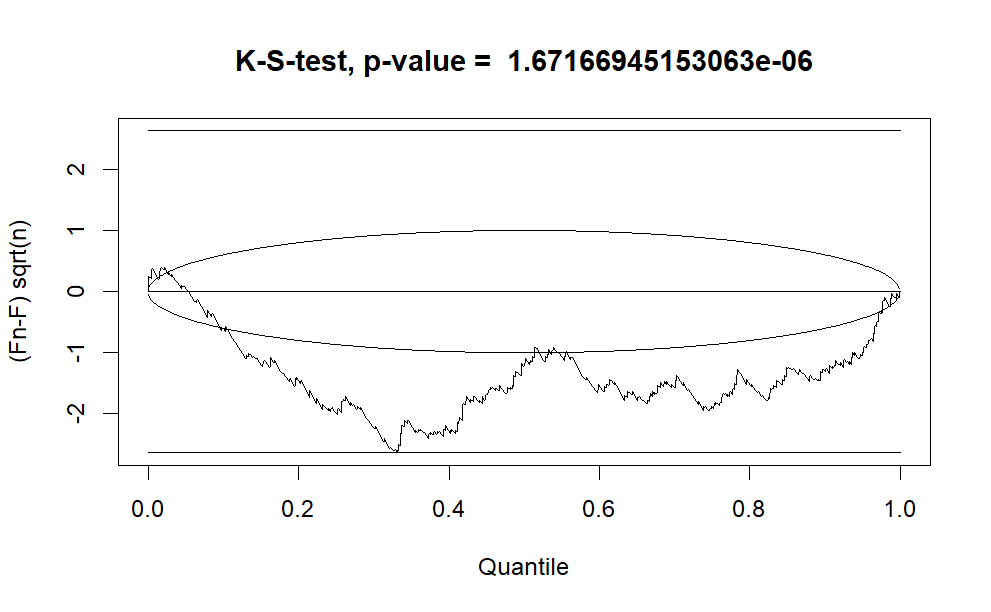
\includegraphics[scale = .6]{2/MSc_LaTeX_SwDS/MSc_LaTeX_SwDS/ks_org_best.png}
\caption{KS Plot of Time-between-Events of an Organic Catalogue}
\label{fig:ks_org}
\end{figure}

\begin{figure}[h]
\centering
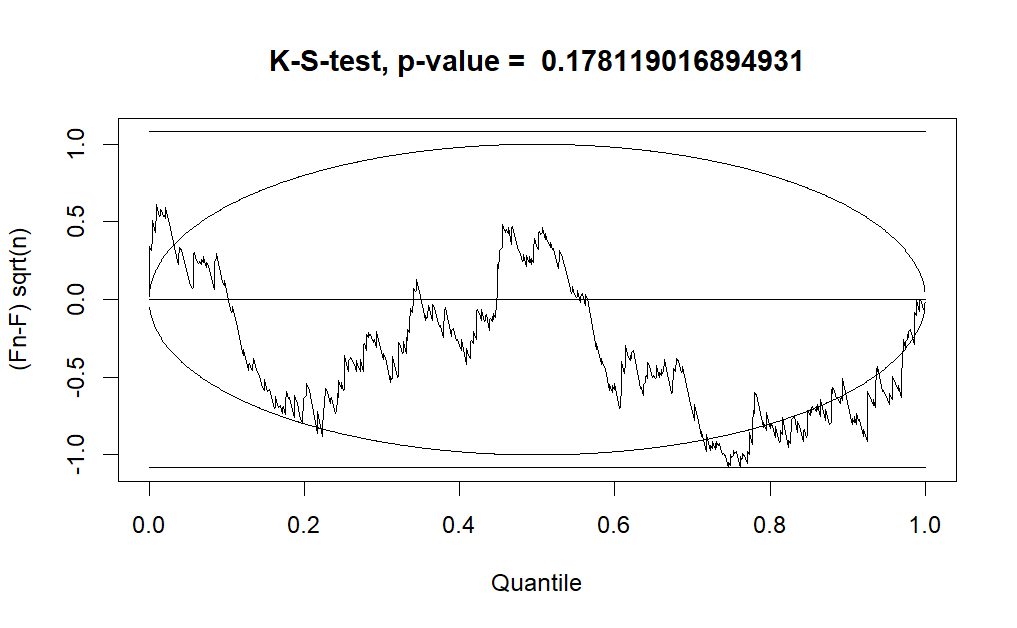
\includegraphics[scale = .6]{2/MSc_LaTeX_SwDS/MSc_LaTeX_SwDS/ks_imp_best.png}
\caption{KS Plot of Time-between-Events of a Catalogue with Imposed History}
\label{fig:ks_imp}
\end{figure}
\clearpage
\section{Conclusions}

From this project, $3$ conclusions could be drawn in mimicking the characteristics of the L'Aquila sequence. In terms of sensitive parameters, it is suggested that the average number of aftershocks triggered, the time offset parameter, and the decaying rate are to be estimated correctly in order to yield better estimation results of other parameters. In terms of key characteristics to be captured, it is suggested that the organic synthetic catalogues with $300$ to $500$ total events, with $3$ to $5$ large events, and with the largest event of magnitude around $6$ would lead to a better performance in mimicking the characteristics of the sequence. Finally, in terms of the time-between-events, it is suggested that imposing the largest event to the history has a higher chance to yield a similar behaviour of the real sequence.



%TC:ignore
\clearpage

%the entries have to be in the file literature.bib
\bibliography{literature}
\clearpage

%\appendix
%\section*{Appendices}
%\addcontentsline{toc}{section}{Appendices}

%\section{An Appendix}
%\label{app:one}

%Some stuff.

%\begin{lstlisting}[language = R]

%\end{lstlisting}

%\clearpage

%\section{Another Appendix}
%\label{app:two}

%Some other stuff.
%TC:endignore
\end{document}
